%%%%%%%%%%%%%%%%%%%%%%%%%%%%%%%%%%%%%%%%%%%%%%%%%%%%%%%%%%%%%%%%%%%%%%%%%%%%%%%%%%%%%%%%%%%%%%%%
%
% CS484 Written Question Template
%
% Acknowledgements:
% The original code is written by Prof. James Tompkin (james_tompkin@brown.edu).
% The second version is revised by Prof. Min H. Kim (minhkim@kaist.ac.kr).
%
% This is a LaTeX document. LaTeX is a markup language for producing 
% documents. Your task is to fill out this document, then to compile 
% it into a PDF document. 
%
% 
% TO COMPILE:
% > pdflatex thisfile.tex
%
% If you do not have LaTeX and need a LaTeX distribution:
% - Personal laptops (all common OS): www.latex-project.org/get/
% - We recommend latex compiler miktex (https://miktex.org/) for windows,
%   macTex (http://www.tug.org/mactex/) for macOS users.
%   And TeXstudio(http://www.texstudio.org/) for latex editor.
%   You should install both compiler and editor for editing latex.
%   The another option is Overleaf (https://www.overleaf.com/) which is 
%   an online latex editor.
%
% If you need help with LaTeX, please come to office hours. 
% Or, there is plenty of help online:
% https://en.wikibooks.org/wiki/LaTeX
%
% Good luck!
% Min and the CS484 staff
%
%%%%%%%%%%%%%%%%%%%%%%%%%%%%%%%%%%%%%%%%%%%%%%%%%%%%%%%%%%%%%%%%%%%%%%%%%%%%%%%%%%%%%%%%%%%%%%%%
%
% How to include two graphics on the same line:
% 
% \includegraphics[\width=0.49\linewidth]{yourgraphic1.png}
% \includegraphics[\width=0.49\linewidth]{yourgraphic2.png}
%
% How to include equations:
%
% \begin{equation}
% y = mx+c
% \end{equation}
% 
%%%%%%%%%%%%%%%%%%%%%%%%%%%%%%%%%%%%%%%%%%%%%%%%%%%%%%%%%%%%%%%%%%%%%%%%%%%%%%%%%%%%%%%%%%%%%%%%

\documentclass[11pt]{article}

\usepackage[english]{babel}
\usepackage[utf8]{inputenc}
\usepackage[colorlinks = true,
            linkcolor = blue,
            urlcolor  = blue]{hyperref}
\usepackage[a4paper,margin=1.5in]{geometry}
\usepackage{stackengine,graphicx}
\usepackage{fancyhdr}
\setlength{\headheight}{15pt}
\usepackage{microtype}
\usepackage{times}
\usepackage{booktabs}

% From https://ctan.org/pkg/matlab-prettifier
\usepackage[numbered,framed]{matlab-prettifier}

\frenchspacing
\setlength{\parindent}{0cm} % Default is 15pt.
\setlength{\parskip}{0.3cm plus1mm minus1mm}

\pagestyle{fancy}
\fancyhf{}
\lhead{Homework Writeup}
\rhead{CS484}
\rfoot{\thepage}

\date{}

\title{\vspace{-1cm}Homework 4 Writeup}


\begin{document}
\maketitle
\vspace{-3cm}
\thispagestyle{fancy}

\section*{Instructions}
\begin{itemize}
  \item Describe any interesting decisions you made to write your algorithm.
  \item Show and discuss the results of your algorithm.
  \item Feel free to include code snippets, images, and equations.
  \item Use as many pages as you need, but err on the short side If you feel you only need to write a short amount to meet the brief, th
  
  \item \textbf{Please make this document anonymous.}
\end{itemize}
\newcommand\tab[1][1cm]{\hspace*{#1}}
\section*{Files}

{\large $1.$ get\_tiny\_image.m \par}
\tab input : image\_path \\
\tab output : image\_feats 

{\large $2.$ nearest\_neighbor\_classify.m \par}
\tab input : train\_image\_feats, train\_labels, test\_image\_feats \\
\tab output : predicted\_categories 

\tab $1.$ and $2.$ are the first section.\\

{\large $3.$ bulid\_vocabulary.m \par}
\tab input : image\_paths, vocab\_size \\
\tab output : vocab

{\large $4.$ get\_bags\_of\_words.m \par}
\tab input : image\_paths \\
\tab output :  image\_feats 

\tab $2.$ and $3.$\&$4.$ are the second section.\\

{\large $5.$ svm\_classify.m \par}
\tab input : train\_image\_feats, train\_labels, test\_image\_feats \\
\tab output : predicted\_categories 

\tab $5.$ and $3.$\&$4.$ are the last section.\\

\section*{Code}
{\large $1.$ get\_tiny\_image.m \par}
\begin{lstlisting}[style=Matlab-editor]
N = size(image_paths,1);
image_feats = zeros(N,256);
for i = 1:N
    resize_im = imresize(imread(image_paths{i}),[16 16]);
    image_feats(i,:) = reshape(resize_im, 1,256);
    image_feats(i,:) = image_feats(i,:) - mean(image_feats(i,:));
    image_feats(i,:) = image_feats(i,:)./norm(image_feats(i,:));
end
\end{lstlisting}

This function resizes the size of the image. Afterwards, the image is corrected by dividing it into norm.\\

{\large $2.$ nearest\_neighbor\_classify.m \par}
\begin{lstlisting}[style=Matlab-editor]
N1 = size(test_image_feats,1);
D = pdist2(train_image_feats,test_image_feats);
k = 15;
label = unique(train_labels);
size_l = size(label,1);
[~, index] = sort(D,1);
count = zeros(size_l,N1);
for i = 1:N1
    for j = 1:size_l
        m = train_labels(index(1:k,i));
        count(j,i) = sum(strcmp(label(j),m));
    end
end
[~, index_l] = max(count,[],1);
predicted_categories = label(index_l);
end 
\end{lstlisting}

It is first method to categorize the images. Nearest neighbor classifier.\\



\newpage
{\large $3.$ bulid\_vocabulary.m \par}
\begin{lstlisting}[style=Matlab-editor]
N1 = size(image_paths,1);
feat = [];
for i = 1:N1
    I1 = im2single(imread(image_paths{i}));
    SURF = detectSURFFeatures(I1);
    strongest = SURF.selectStrongest(200);
    [features,v] = extractHOGFeatures(I1,strongest,'CellSize',[48 48]);
    size_f = size(features,1);
    rand1 = randperm(size_f);
    sample = rand1(1:round(size_f/5));
    other = features(sample,:);
    feat = vertcat(feat,other);
end
[idx,C] = kmeans((feat),vocab_size);
vocab = C;
\end{lstlisting}

Catch the feature with the fuction extractHOGFeatures. It makes vocab.mat to find feature at get\_bags\_of\_words.m.\\

\newpage
{\large $4.$ get\_bags\_of\_words.m \par}
\begin{lstlisting}[style=Matlab-editor]
load('vocab.mat')
size_v = size(vocab, 1);
N = size(image_paths, 1);
image_feats = zeros(N, size_v);
for i=1:N
    I1 = im2single(imread(image_paths{i}));
    SURF = detectSURFFeatures(I1);
    strongest = SURF.selectStrongest(200);
    [features,v] = extractHOGFeatures(I1,strongest,'CellSize',[48 48]);
    temp = zeros(size_v,1);
    index = knnsearch(vocab,features,'K',23);
    size_i=size(index,1);
    for j=1:size_i
        for k=1:10
            temp(index(j,k)) = temp(index(j,k)) +1;
        end
    end
    hist = temp./norm(temp);
    image_feats(i,:) = hist;
end
\end{lstlisting}

Categorize the images with knn algorithm.\\
I find $K$ value with experiment. $(K=23)$
\newpage
{\large $5.$ svm\_classify.m \par}
\begin{lstlisting}[style=Matlab-editor]
categories = unique(train_labels);
num_categories = length(categories);

scores = [];
for i=1:num_categories
    match = strcmp(categories{i},train_labels);
    
    % fitcl =fitclinear(train_image_feats,match');
    fitcl = fitcsvm(train_image_feats,match');
    W = fitcl.Beta';
    B = fitcl.Bias;
    predict = W*test_image_feats'+B;
    scores = [scores; predict];
end

[M,I] = max(scores);
predicted_categories = categories(I);
end
\end{lstlisting}

Categorize the images with svm algorithm.
\newpage
\section*{Result}
\begin{figure}[!h]
    \centering
    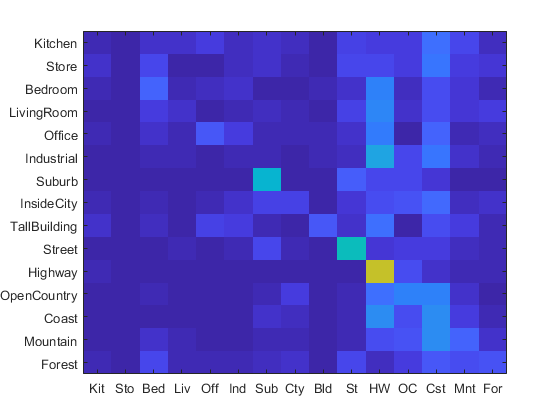
\includegraphics[width=8cm]{image1.png}
    \caption{tiny image\&nearest neighbor}
    \label{fig:result1}
\end{figure}
section $1.$ \\
FEATURE = 'tiny image'\\
CLASSIFIER = 'nearest neighbor'\\
Accuracy = 0.221\\
\\
\begin{figure}[!h]
    \centering
    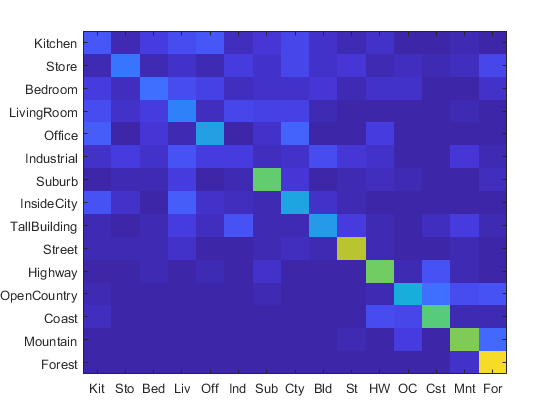
\includegraphics[width=8cm]{image2.png}
    \caption{bag of words\&nearest neighbor}
    \label{fig:result2}
\end{figure}
section $2.$ \\
FEATURE = 'bag of words'\\
CLASSIFIER = 'nearest neighbor'\\
Accuracy = 0.448\\
\\
\newpage
\begin{figure}[!h]
    \centering
    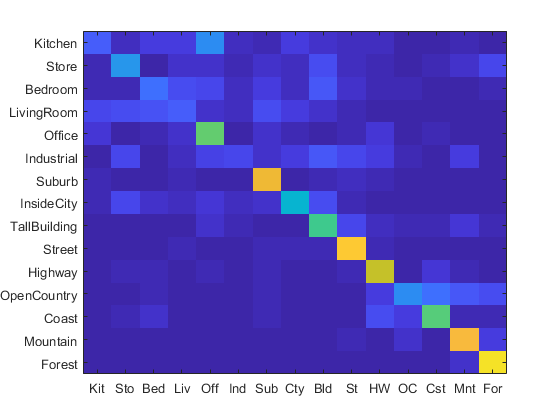
\includegraphics[width=8cm]{image3.png}
    \caption{bag of words\&support vecter machine}
    \label{fig:result3}
\end{figure}
section $3.$ \\
FEATURE = 'bag of words'\\
CLASSIFIER = 'support vecter machine'\\
Accuracy = 0.518\\
\\
\end{document}